% !TeX spellcheck = en_US
\documentclass[french]{yLectureNote}

\title{Électromagnétisme 1 PS}
\subtitle{Physique}
\author{Paulhenry Saux}
\date{\today}
\yLanguage{Français}
%lionels.calmels@cemes.fr
\professor{F.Pettinari}
\usepackage{graphicx}%----pour mettre des images
\usepackage[utf8]{inputenc}%---encodage
\usepackage{geometry}%---pour modifier les tailles et mettre a4paper
%\usepackage{awesomebox}%---pour les boites d'exercices, de pbq et de croquis ---d\'esactiv\'e pour les TP de PC
\usepackage{tikz}%---pour deiffner + d\'ependance de chemfig
% \usepackage{tabularx}%---pour dimensionner automatiquement les tableaux avec variable X
\usepackage{awesomebox}%---Pour les boites info, danger et autres
\usepackage{menukeys}%---Pour deiffner les touches de Calculatrice
\usepackage{fancyhdr}%---pour les en-t\^ete personnalis\'ees
\usepackage{blindtext}%---pour les liens
\usepackage{hyperref}%---pour les liens (\`a mettre en dernier)
\usepackage{caption}%---pour la francisation de la l\'egende table vers Tableau
\usepackage{pifont}
\usepackage{array}%---pour les tableaux
\usepackage{lipsum}
\usepackage{yFlatTable}
\usepackage{multicol}
\newcommand{\Lim}[1]{\lim\limits_{\substack{#1}}\:}
\renewcommand{\vec}{\overrightarrow}
\newcommand{\N}[0]{\mathbb{N}}
\newcommand{\dd}{\mathrm{d}}
\newcommand{\norm}[1]{||\vec{#1}||}
\newcommand{\fo}{\psi(\vec{r},t)}
\newcommand{\foe}{\psi(\vec{r},t)\*}
\newcommand{\HH}{\hat{H}}
\newcommand{\hb}{\hbar}
\newcommand{\lap}{\nabla^2}
\newcommand{\lapcc}{\frac{\partial^2 }{\partial x^2}+\frac{\partial^2 }{\partial y^2}+\frac{\partial^2 }{\partial z^2}}
\newcommand{\E}{\vec{E}(M)}
\newcommand{\B}{\vec{B}(M)}
\newcommand{\V}{V(M)}
\newcommand{\er}{\vec{e_{\rho}}}
\newcommand{\ep}{\vec{e_{\varphi}}}
\newcommand{\pip}{\pi^+}
\newcommand{\pim}{\pi^-}
\newcommand{\mv}{\mathcal{V}}
\begin{document}
\setcounter{chapter}{6}

\chapter{Champ magnétique : Biot et Savart}
\section{Champ \(\vec{B}(M)\) créé par un fil}
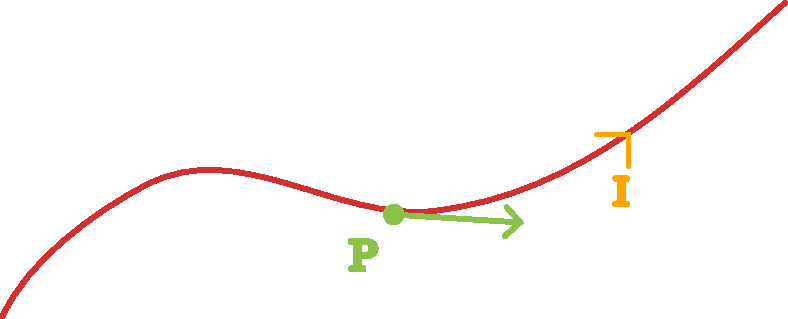
\includegraphics[scale=0.5]{fil}

On suppose un champ \(\B\) crée par un fil d'épaisseur négligeable parcourue par un courant électrique d'intensité I\marginCheck[Rappel]{I est algébrique}. On note P un point du fil électrique, et \(\vec{\dd l(P)}\) le long du fil électrique, orienté dans le sens du courant au point P.

M est le point pour lequel on veut calculer le champ magnétique crée par ce courant.

On admettra que le fil  de longueur élémentaire \(\dd l(P)\) parcourue par le courant d'intensité I crée en M le champ magnétique élémentaire :
\begin{theorem}[Champ magnétique élémentaire d'un fil]
 \[\dd \B = \frac{\mu_0}{4\pi} \frac{I \vec{\dd l}(P)\wedge \vec{PM}}{\norm{PM}^3}\] avec \(\mu_0 = 4\pi \cdot 10^{-7}\)
\end{theorem}
On remarque \(\norm{\dd \B}\) décroît en \(\frac{1}{\norm{PM}^2}\)

La dimension est de \(\vec{\dd \B}\) est \(\frac{[\mu_0]I}{L}\).

On n' a plus qu'à faire l'intégrale :
\begin{theorem}[Loi de Biot et Savart]
 \[\B = \frac{\mu_0}{4\pi}  \int_{P\in F} \frac{I\vec{\dd l}(P)\wedge \vec{PM}}{\norm{PM}^3}\]
\end{theorem}
%TODO Vérifier la puissance au dénomnateur


% L'intégrale porte sur la coordonnée du point P permettant de repérer sa position sur le fil.
\section{Distribution surfacique}
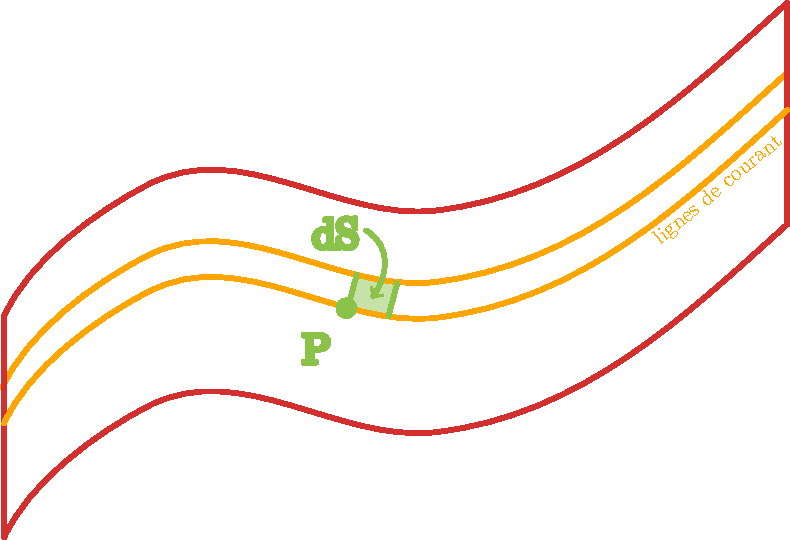
\includegraphics[scale=0.4]{surface}

On considère un ruban parcouru par une densité surfacique de courant. P est un point sur le ruban. On note \(\dd S(P)\) située au point P et délimitée par des lignes de courant. \(j_s(P)\) est la densité surfacique de courant au point P. Sur \(\dd S(P)\), \(j_s\) est considéré uniforme sur la surface.

% Le champ magnétique élémentaire crée en M  est \[\dd \B = \frac{\mu_0}{4\pi}\frac{\dd S \vec{j_s}(P)\wedge \vec{PM}}{\norm{PM}^3}\]
%
% On n' a plus qu'à intégrer :
On obtient
\[\B = \iint_{P\in S} \frac{\mu_0}{4\pi}\frac{\dd S \vec{j_s}(P)\wedge \vec{PM}}{\norm{PM}^3}\]
\section{Distribution volumique de courant}
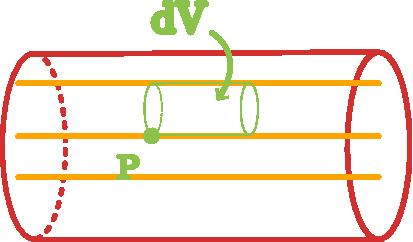
\includegraphics[scale=0.4]{volume}

De la m\^eme façon, P est un point dans le câble, \(\vec{j_p}\) la densité volumique de courant au point P. \(\dd \mv\) est le volume élémentaire délimité latéralement par des lignes de courant. On obtient \[\B = \iiint_{P\in \mv} \frac{\mu_0}{4\pi}\frac{\dd \mv \vec{j}(P)\wedge \vec{PM}}{\norm{PM}^3}\]
\section{Exemples}
\subsection{Fil infiniment long}
La distribution de courant est à symétrie cylindrique autour du fil d'axe Oz, M est repéré par ses coordonnées cylindriques dans la base cylindrique locale. La position de P sur le fil est repérée par \(z_p\) et on  a \(\vec{\dd l}(P) = \dd z_p \vec{e_z}\).

On écrit \(\vec{PM} = -z_p\vec{e_z}+ (\rho \er+z\vec{e_z})\)

Il y a invariance par translation selon \(e_z\) du courant. Pour simplifier, on peut faire le calcul en mettant M dans le plan \(Oxy\).  On a donc \(\vec{PM} = -z_p\vec{e_z}+\rho \er\).

On écrit :
\explanation{1}{On utilise la primitive vue en TD et on l'évalue aux limites en \(\pm \infty\)}
\begin{flalign*}
\dd \B &= \frac{\mu_0}{4\pi} \frac{I\dd z_p \vec{e_z}\wedge (-z_p\vec{e_z}+\rho \er)}{(z_p^2+\rho^2)^{3/2}}\\
&=  \frac{\mu_0}{4\pi} \frac{\rho I \dd s_p \ep}{(z_p^2+\rho^2)^{3/2}}\\
&\Rightarrow \B = \int^{\infty}_{-\infty} \dd \B\\
& = \frac{\mu_0 I\rho}{4\pi}\ep \int \frac{\dd z_p}{(z_p^2+\rho^2)^{3/2}}\\
&= \frac{\mu_0 I\rho}{4\pi}\ep \frac{2}{\rho^2}\explain{1}{right}{0}{0.5}{} \\
&= \frac{\mu_0 I}{2\pi \rho}\ep
\end{flalign*}
\begin{proposition}[Champ crée par un fil infiniment long]
\[\vec{B}(M) = \frac{\mu_0 I}{2\pi \rho}\vec{e_{\varphi}}\]
\end{proposition}

Le champ est toujours selon \(\ep\), donc orthoradial et les lignes de champ sont circulaires\marginInfo{Si I est négatif, les lignes sont orientées dans le sens opposé.}.
\subsection{Spire circulaire}
% On cherche maintenant le champ crée par une spire circulaire crée en un point M placé sur l'axe de la spire.

Compte tenu des symétries autour de  l'axe de la spire, on écrit P avec ses coordonnées cylindriques dans la base locale. On a \(\dd l(P) = R\dd \varphi_p \vec{e_{\varphi_P}} \). De plus, \(\vec{PM} = - R\vec{e_{\varphi_P}}+z\vec{e_z})\). En injectant dans la loi de Biot et Savat :
\begin{flalign*}
\dd \B &= \frac{\mu_0}{4\pi}  \frac{IR \dd \varphi_P \vec{\varphi_P}(-R \vec{e_{\varphi_P}}+z\vec{e_z})}{(R^2+z^2)^{3/2}}\\
&= \frac{\mu_0 IR \dd \varphi_{P}}{4\pi (R^2+z^2)^{3/2}}(R\vec{e_z}+z\vec{e_{\rho_P}})
\end{flalign*}
On remarque qu'il y a 2 composantes, et non seulement une composante selon \(\vec{e_z}\) !

Cependant, on voit géométriquement que 2 point diamétralement opposés forment une somme de db dont la composante selon \(\er\) s'annule.


\includegraphics[scale=0.5]{symetrie}

Donc on peut garder que la composante selon \(\vec{e_z}\) pour le calcul intégral.

On a donc \[\B = \frac{\mu_0IR^2}{2(R^2+z^2)^{3/2}}\vec{e_z}\]

% On remarque que cela tend vers 0 en \(z^{-3}\). De plus, la fonction est paire car \(z^2\).
\checkInfo{Remarque : Autre expression de B}{On a \(\B = \frac{\mu_0 I}{2R}\sin^3(\alpha)\vec{e_z}\) avec \(\alpha\) l'angle sous lequel on voit la spire depuis M. En effet, \(\sin(\alpha) = \frac{R}{(R^2+z^2)^{1/2}}\)

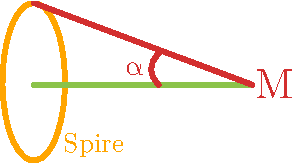
\includegraphics[scale=0.5]{spire}
}
\begin{proposition}[Champ pour une spire]
\[\B = \frac{\mu_0 I}{2R}\sin^3(\alpha)\vec{e_z}\] avec \(\alpha\) l'angle sous lequel on voit la spire depuis M.
\end{proposition}

% \chapter{Propriétés de B}
% \section{Théorème de superposition}
% Le champ magnétique crée par un ensemble de distribution de courant vaut la somme de tout ces champs  crées par une distribution.
% \section{Direction de B}
% Vérifie les propriétés du produit vectoriel
\section{Conséquence des symétries de la Distribution de courant}
\begin{center}
\begin{tabular}{ll}
Situation & Direction\\
M \(\in \pip\) & B est \(\perp\) au plan\\
M \(\in \pim\) & B est contenu dans le plan\\
\( (Oxy) \in  \pip\) & Selon z, \(B_z\) paire, \(Bx,B_y\) impaires\\
\( (Oxy) \in  \pim\) & Selon z, \(B_z\) impaire, \(Bx,B_y\) paires
\end{tabular}
\end{center}
En effet, Le champ magnétique est relié à ses sources (courants électriques) via la loi de Biot et Savart, qui contient un produit vectoriel. In en résulte que le champ appartient à la famille des Pseudo vecteurs, qui ont la propriété d'\^etre contenus dans les plans d'antysmétrie de leurs sources et ortogonaux aux plan de symétrie de leur sources.
% \subsection{Direction de \(\B\) en un point appartenant à un \(\pip\)}
% % Rappel : Plan \(\pip\) : Dans ces cas, les extrémités des vecteurs sont également symétriques l'un de l'autre par rapport au plan \(\pip\).
%
% On a donc  \(I\vec{\dd l}(P_1) = I\vec{\dd l}(P_2)\). En injectant dans la loi de Biot et Savart, on  a \(\norm{\dd B_1(M)} = \norm{\dd B_2(M)}\)
%
% Or, on sait que \[\vec{\dd B_1(M)} = \frac{\mu_0}{4\pi}\frac{I\vec{\dd l}(P_1)\wedge \vec{P_1M}}{\norm{P_1M}^3}\] et
% \[\vec{\dd B_2(M)} = \frac{\mu_0}{4\pi}\frac{I\vec{\dd l}(P_2)\wedge \vec{P_2M}}{\norm{P_2M}^3}\]
%
% Note : BOUUUUH.
%
% On peut tracer les 2 vecteurs obtenus : on se rend compte que la résultante est ortogonale au plan \(\pip\) passant par M.
%
% Règle générale : si un point M appartient à un plan de symétrie , alors le champ magnétique est perpendiculaire au plan de symétrie passant par M.
%
% \subsection{Direction de B en un point M contenu dans un plan \(\pim\)}
% Ici, les courants élémentaires sont rigoureusement opposés, de m\^eme norme.
%
% Avec les m\^emes raisonnements que précédement, on obtient cette fois ci que
%
% Règle générale : si un point M appartient à un plan de symétrie , alors le champ magnétique est contenu dans le plan d'antisymétrie passant par M.
%
% Si plusieurs plans \(\pim\) passent par M, alors B appartient à leur intersection.
% \subsection{Notion de Pseudo-vecteur/vecteur axial}
% Le champ magnétique est relié à ses sources (courants électriques) via la loi de Biot et Svaart contenant un produit vectoriel. In en résulte que le champ appartient à la famille des Pseudo vecteurs, qui ont la propriété d'\^etre contenus dans les plans d'antysmétrie de leurs sources et ortogonaux aux plan de symétrie de leur sources.
% \section{Propriétés de parité et d'imparité des composantes de B}
% \subsection{Cas d'un plan \(\pip\) ne passant pas par M}
% On prend en example un plan \(\pip\) Oxy et 2 points \(M(z), M'(-z)\)
%
% Bilan : Si (Oxy) = \(\pip\), alors \(B_z(x,y,z) = B_z(x,y,-z), B_x(x,y,z) = - B_x(x,y,-z), B_y(x,y,z) = - B_y(x,y,-z)\)
% \subsection{Plan \(\pim\) ne passant pas par M}
% Bilan : Si (Oxy) = \(\pip\), alors \(B_z(x,y,z) = -B_z(x,y,-z), B_x(x,y,z) =  B_x(x,y,-z), B_y(x,y,z) =  B_y(x,y,-z)\)
%
% En effet, \(\norm{P_1M} = \norm{P_2M'}, \norm{P_1M'} = \norm{P_2M}\)
\section{Exemples}
\subsection{Spire circulaire}
\subsubsection{Analyse générale}
\begin{itemize}
 \item Cette distribution de courant est à symétrie cylindrique autour de l'axe de la spire, donc on repère un point M par ses coordonnées cylindriques dans la base cylindrique locale.
 \item De plus, le plan \((M, \er, \vec{e_z})\) est un plan \(\pim\) passant par M. Or \(\B\) est pseudo-vecteur, donc il appartient à ce plan.
 \item Donc \(\vec{B} = B_{\rho}\er + B_z \vec{e_z}\).
 \item Invariances : Invariance par rotation autour de l'axe z, donc \(\vec{B} = B_{\rho}(\rho, z)\er + B_z(\rho, z) \vec{e_z}\).
\item Parité/Imparité : (Oxy) est un plan \(\pip\), donc \(B_z(z) = B_z(-z), B_{\rho}(z) = -B_{\rho}(-z)\)
\end{itemize}
\subsubsection{Cas particuliers}
Cas paticulier 1 : Si \(M\in (Oxy)\), le plan est un plan \(\pip\) passant par M, donc \(B\perp\) à ce plan, donc \(\vec{B} = B_z\vec{e_z}\).

Cas particulier 2 : Si \(M\in (Oz)\) Tous les plans contenants Oz sont des \(\pim\) passants par M, donc le champ est dans leur intersection et \(\vec{B} = B_z\vec{e_z}\)

% On peut utiliser ces informations pour trouver les lignes de champ de B :
%
% De plus, on doit respecter la symétrie de révolution autour de Oz.
% %TODO Ligne de champ

% \subsection{Fil rectiligne infiniment long}
% La distribution est à symétrie cylindrique autour du fil, donc Oz est l'axe du fil, O est n'importe où.
%
% Plans \(\pim\) : \((M, \er, \ep)\), Plan \(\pip\) : \((M, \er, \vec{e_z})\).
%
% Mais B est un pseudo-vecteur, perpendiculaire au plan \(\pip\) passant par M, donc \(\vec{B} = B_{\varphi} \ep\).
%
% Avec les invariances (ici de rotation autour de Oz, et de translation selon Oz), on trouve finalament, par le principe de curie :
% \(\vec{B} = B_{\varphi}(\rho) \ep\)
% \chapter{Calcul de B avec Ampère}
% Cette méthode de calcul du champ magnétique ne peut \^etre exploitée que dans les rares cas où la distribution de courant est hautement symétrique.
% \section{Démonstration}
% On prend un fil rectiligne infiniment long parcourue par un courant d'intensité I.
%
% On a déjà montré que \[\B = \frac{\mu_0 I}{2\pi\rho}\ep\]
%
% \begin{enumerate}
%  \item On montre que la circulation  de \(\B\) sur 1 circuit fermé circulaire d'ace Oz vaut \(\mu_0I\) que que soit ce circuit, si on oriente dans le sens positif :
%
%  On choisit d'orienter \(\dd l\) dans le sens positif choisi.
%
%  On écrit \[\int \B \cdot  \vec{\dd l} = \int_{\varphi = 0}^{2\pi} \ep \cdot \rho \dd \varphi \ep = \frac{\mu_0I}{2\pi}\cdot 2\pi = \mu_0I \]
%
%  \item On montre que la circulation  de \(\B\) sur 1 circuit fermé circulaire d'ace Oz vaut \(-\mu_0I\) que que soit ce circuit, si on oriente dans le sens négatif :
%
%  On fait la meme chose que précédement, sauf qu'on tourne dans le sens anti-trigonométrique, donc on va vers -\(2\pi\) et on trouve le bon résultat.
%
%  \item On montre que la circulation de B sur un contour fermé n'enlançant pas le courant est nulle.
%
%  On choisit le contour d' un morceau de Donut comme chemin. Les résultats des chemins opposés se compensent ou sont nuls par les propriétés du produit scalaire
% \end{enumerate}
% \section{Énoncé du théorème d'Ampère}
 \end{document}
